\chapter{\texorpdfstring{Nb$_3$Sn}{Nb3Sn} for High-Field Applications}\label{sec:whynb3sn}

As discussed earlier, axion detection experiments could achieve faster scanning of the exploration space by using superconducting RF cavities operating in multi-tesla magnetic fields. This chapter examines the merits of  Nb$_3$Sn for this application.

\section{\texorpdfstring{Nb$_3$Sn}{Nb3Sn} vs Other Superconducting Materials}

Nb$_3$Sn is the most technologically mature high-field superconductor other than NbTi alloy. Among strongly type~II superconductors (NbTi, Nb$_3$Sn, REBCO, BSCCO), Nb$_3$Sn offers the optimal balance of properties for RF cavity applications~\cite{gurevichUseNotUse2011}. Its high critical temperature and upper critical field ($T_c = 18.3$~K and $H_{c2} = 30$~T) exceed NbTi's capabilities, while its larger coherence length ($\xi_0 \sim 3$~nm) compared to high-temperature superconductors such as REBCO ($\xi_0\sim 1{-}2$~nm), reduce grain boundary resistance~\cite{gurevichUseNotUse2011}. When the coherence length ($\xi_0$) becomes smaller than typical grain boundary widths ($\sim3{-}5$~nm), supercurrent cannot cross grain boundaries coherently, causing severe weak-link behavior and increased dissipation~\cite{alexgurevich33ThermalRF2006}. Nb$_3$Sn's coherence length ($\xi_0 \approx$ GB width) makes grain boundary quality important, but it is potentially manageable with proper processing. In contrast, REBCO's much smaller $\xi_0 \ll$ GB width means grain boundaries act as intrinsic weak links regardless of processing. High-temperature superconductors also exhibit strong crystalline anisotropy, leading to properties varying dramatically with crystal orientation. This may lead to degraded properties for unfavorable orientations of the magnetic field. Table~\ref{tab:SC_comparison} summarizes key superconductor properties of relevant superconducting materials.



\begin{table}[ht]
    \centering
    \caption{Comparison of superconductor properties relevant for high-field RF applications}
    \begin{tabular}{lcccc}
    \hline
    Material & Type & $T_c$ (K) & $H_{c2}$ (0 K, T) & $\xi_0$ (nm) \\
    \hline
    Nb & LTS & 9.2 & 0.4 & 40 \\
    NbTi & LTS & 9.1 & 11.3 & 5.2 \\
    Nb$_3$Sn & LTS & 18.3 & 30 & 3 \\
    REBCO$^*$ & HTS & 93 & $>$100 & $\sim$1.5$^{**}$ \\
    BSCCO$^*$ & HTS & 110 & $>$100 & $\sim$2$^{**}$ \\
    \hline
    \multicolumn{5}{l}{\small $^*$REBCO = REBa$_2$Cu$_3$O$_{7-x}$ (RE = rare earth element)} \\
    \multicolumn{5}{l}{\small \hspace{0.5em} BSCCO = Bi$_2$Sr$_2$Ca$_2$Cu$_3$O$_{14+x}$} \\
    \multicolumn{5}{l}{\small $^{**}$In-plane coherence length; c-axis values are 3-10× smaller}
     \end{tabular}
    \label{tab:SC_comparison}
\end{table}

Nb$_3$Sn benefits from decades of optimization by the high-field magnet community, with thousands of established magnets delivered to customers~\cite{cooleyBusinessModelsAssure2023}. The accelerator community is also pursuing Nb$_3$Sn cavities to surpass Nb's fundamental accelerating gradient limit of 50~MV/m. However, as an intermetallic compound rather than a ductile metal or alloy, Nb$_3$Sn requires fundamentally different fabrication approaches than those used for most cavity resonators. Traditional metal-forming and welding techniques cannot be applied to intermetallic structures because these materials are brittle and prone to cracking. A wide range of opportunities for fabricating axion detector cavities is afforded by thin-film deposition onto suitable substrates. Similar opportunities exist for other high-field intermetallic superconductors.

\section{Fundamental Material Properties of \texorpdfstring{Nb$_3$Sn}{Nb3Sn}}
 
    \subsection{Crystal Structure (A15)}

    The stoichiometry of Nb$_3$Sn is 3:1 (Nb:Sn), corresponding to 75 at.\% Nb and 25 at.\% Sn. It is part of a class of materials called A15 compounds. All of these materials have a chemical composition of A${_3}$B, where A is a transition metal, and B is any element. Many of these materials have surprisingly good superconducting properties, with high $T_c$ and $H_{c2}$. The Nb atoms couple up in twos, forming linear chains along the alternating faces of a cubic unit cell. The Sn atoms occupy a body-centered cubic (BCC) position, as shown in Fig.~\ref{fig:CrystalStructure}. These aligned Nb chains facilitate electron transport between unit cells. This cubic unit cell leads to isotropic superconducting properties, unlike HTS materials. 
    
    %When dopants replace Sn sites (such as Ti, Hf, or Ta), $T_c$ remains relatively constant. However, when elements replace Nb sites, $T_c$ typically decreases, highlighting the critical role of the Nb chains in superconductivity.
    
    \begin{figure}[H]   
        \centering
        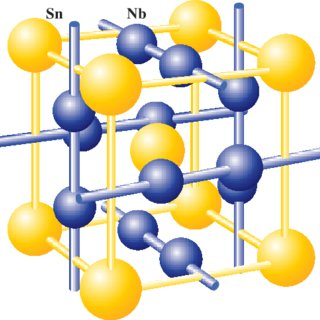
\includegraphics[width=.5\textwidth]{images/Nb3Sn/CrystalStructure.png}
        \caption{Arrangement of Nb and Sn atoms in Nb$_3$Sn crystal structure~\cite{godekeReviewPropertiesNb3Sn2006}.}
        \label{fig:CrystalStructure}
    \end{figure}

    \subsection{Nb-Sn Phase Diagram}
  
    The Nb$_3$Sn compound can form with a varying degree of Sn\%, from 16 to 26~at.\% Sn, where 25~at.\% Sn is the most desirable for superconducting properties~\cite{devantayPhysicalStructuralProperties1981}. There are other Nb-Sn compounds, Nb$_6$Sn$_5$ and NbSn$_2$, with poor superconducting properties ($T_c = 2.8$ K, and $T_c = 2.68$ K respectively). These compounds can form when reacting Nb and Sn at temperatures below 930~$^\circ$C (Fig.~\ref{fig:NbSnphasediagram})~\cite{charlesworthExperimentalWorkNiobiumtin1970}.

     \begin{figure}[H]   
        \centering
        
\includegraphics[width=.7\textwidth]{images/intro/Nb3SnProperties/NbSnphasediagram.png}
        \caption{Nb-Sn Phase diagram, where the Nb$_3$Sn compound is highlighted in yellow, and above the purple line shows where Nb$_6$Sn$_5$ and NbSn$_2$ break down~\cite{charlesworthExperimentalWorkNiobiumtin1970}.}
        \label{fig:NbSnphasediagram}
    \end{figure}

    \FloatBarrier
    
    \subsection{Nb-Cu-Sn Reactions}\label{sec:NbCuSn}

    Adding Cu to a Nb-Sn reaction enables Nb$_3$Sn formation at lower temperatures (650--750~°C instead of $>$930~°C). Understanding this ternary reaction requires examining both the Cu-Sn binary system (Fig.~\ref{fig:CuSnPhasediagram}) and the Nb-Cu-Sn ternary diagram (Fig.~\ref{fig:CuSnNbTernaryPhaseDiagram}). Because Cu and Sn have much lower melting temperatures than Nb, Cu-Sn phases form first during heating before reacting with Nb.
    
    The ternary phase diagram reveals which compositions lead to Nb$_3$Sn. Tie lines indicate phases that coexist in thermodynamic equilibrium at a given temperature. At 675~°C, Nb$_3$Sn is in equilibrium with Cu-Sn phases containing $<$1 to 26~at.\% Sn (corresponding to the $\alpha$, $\gamma$, and $\epsilon$ Cu-Sn phases) and with Nb$_6$Sn$_5$. This defines the reaction pathway: Cu-Sn alloys within this composition range can react directly with Nb to form Nb$_3$Sn. Starting from Cu-Sn compositions $>$26~at.\% Sn requires intermediate transformations—either to lower-Sn Cu-Sn phases or to Nb$_6$Sn$_5$—before Nb$_3$Sn can form. This pseudo-binary approach (reacting pre-formed Cu-Sn with Nb) is the basis for commercial Nb$_3$Sn wire manufacturing~\cite{ambrosioNb3SnHighField2015}.
    
    \begin{figure}[htb]         
        \centering
        
\includegraphics[width=.6\textwidth]{images/intro/Nb3SnProperties/CuSnPhasediagram.png}
        \caption{The binary Cu-Sn phase diagram~\cite{shimThermodynamicAssessmentCuSn1996}.}
        \label{fig:CuSnPhasediagram}
    \end{figure} 

    \begin{figure}[htb]          
        \centering
        \includegraphics[width=.6\textwidth]{images/intro/Nb3SnProperties/CuSnNbTernaryPhaseDiagram.png.png}
        \caption{Ternary Cu-Nb-Sn phase diagram at 675 $^{\circ}$C isothermal~\cite{neijmeijerTernarySystemNb1987, lachmannThermodynamicRemodellingCu2022}.}
        \label{fig:CuSnNbTernaryPhaseDiagram}
    \end{figure}

    \FloatBarrier
    
    \subsection{Kinetics of \texorpdfstring{Nb$_3$Sn}{Nb3Sn} Formation}

    Nb$_3$Sn forms by a solid-state diffusion reaction. Growth of the Nb$_3$Sn phase at an interface between Cu-Sn and Nb depends on nucleation, followed by continued supply of Sn as Nb$_3$Sn grains grow. However, as the diffusion reaction proceeds, Sn becomes depleted at the reaction front. As the Nb$_3$Sn layer grows, Sn must diffuse from deeper in the Cu-Sn layer to sustain the reaction. Maintaining the 25~at.\% Sn stoichiometric concentration across a Nb$_3$Sn layer, therefore, requires high-Sn activity and a small diffusion path.
        
    If the diffusion path length from the Sn reservoir to the reaction front is short, grain boundary diffusion rapidly supplies Sn, and the resulting Nb$_3$Sn film maintains approximately constant Sn content throughout its thickness. Conversely, long diffusion paths create Sn concentration gradients, with lower Sn content in regions far from the reservoir. Sn activity is also important, where a mild Cu-Sn alloy, such as $\alpha$, sets up a lower concentration difference to drive diffusion than a Cu-Sn compound with higher Sn content, like $\epsilon$. 
    
    The size of the Sn reservoir also determines the extent of reaction completeness. If the Cu-Sn source layer becomes depleted before all Nb has reacted, the film will exhibit spatial non-uniformity with low-Sn content in regions distant from the original reservoir. The Nb$_3$Sn wire magnet community addressed this challenge by minimizing diffusion distances between Sn sources and Nb. The Restacked-Rod-Process (RRP) wire architecture (red data points in Figure~\ref{fig:SnGradient}) demonstrates how reduced diffusion paths minimize Sn compositional gradients.
    
    \begin{figure}[H]         
        \centering
        
\includegraphics[width=.7\textwidth]{images/Nb3Sn/SnGradient.png}
        \caption{Sn composition vs. distance from Nb$_3$Sn/Cu-Sn interface for different wire architectures~\cite{bannoLowtemperatureSuperconductorsNb3Sn2023}.}
        \label{fig:SnGradient}
    \end{figure}
        
    \section{Properties}\label{sec:Tceffectch5}

    The RF properties of Nb$_3$Sn thin films depend strongly on the film microstructure, which determines the critical temperature $T_c$. The maximum critical temperature can be achieved with a stoichiometric Nb$_3$Sn film ($\sim$25~at.\% Sn) under zero strain. Because both strain and Sn content affect the critical temperature, it is challenging to deconvolve their individual contributions to measured $T_c$ values. Microanalysis of the Sn content in the films helps separate these effects.

    Impurities in the film can also affect the RF properties and cannot be fully characterized with critical temperature measurements alone. Impurities can be found in the bulk or near grain boundaries of the film. If the reaction has sufficient time to equilibrate, impurities are expelled from the bulk into the grain boundaries. Understanding the film morphology at nm-scale resolution is essential for correlating final $Q$ measurements with thin-film properties.

    \subsection{Sn Content Effect}

    Only Nb$_3$Sn films with $25{-}26$~at.\% Sn achieve the optimal critical temperature of $T_c = 18.3$~K (Fig.~\ref{fig:TcvsSnMoore}). An example film with $\sim$25~at.\% Sn in the Nb$_3$Sn layer is confirmed with an EDS line scan seen in Fig.~\ref{fig:25SnNb3SnAS011423}.
    
    \begin{figure}[tb]         
        \centering
        
\includegraphics[width=.8\textwidth]{images/intro/Nb3SnProperties/TcvsSnMoore.png}
        \caption[Plot of critical temperature $T_c$ as a function of at. Sn\% in Nb$_3$Sn.]{Plot of critical temperature $T_c$ as a function of at. Sn\% in Nb$_3$Sn. The maximum $T_c$ is associated with at. Sn 25\% to 26\%~\cite{mooreEnergyGaps151979}.}
        \label{fig:TcvsSnMoore}
    \end{figure}  

    \begin{figure}[tb]          
        \centering
        
\includegraphics[width=.8\textwidth]{images/Nb/25SnNb3SnAS011423.png}
        \caption{EDS linescan of Nb$_3$Sn film with 25\% Sn in the Nb$_3$Sn layer.}
        \label{fig:25SnNb3SnAS011423}
    \end{figure}  
    \FloatBarrier

%These strain and Sn \% dependent parameters affect the quality of the Nb$_3$Sn film and must be considered if the film does not have the properties required for the application. A non-exhaustive conceptual model is shown in Figure~\ref{fig:model}, connecting important variables that relate to the properties of the film.  

%\begin{figure}
 %   \centering
 %   \includegraphics[width=\textwidth]{images/intro/model.png}
 %   \caption[Scope of variables at play for thin film fabrication]{Conceptual model of all the variables that relate to the critical temperature of a film and how they relate. The scope of this diagram is too broad for this dissertation, though it is important to know that these factors are present.}
 %   \label{fig:model}
%\end{figure}


    \subsection{Strain Sensitivity}
    
    Nb$_3$Sn's critical temperature is also strongly strain-dependent (Fig.~\ref{fig:TcvsStrain}). With films $100$~nm to 1~\unit{\um} thickness deposited on copper, the coefficient of thermal expansion (CTE) mismatch is the dominant strain contribution after cooling the material below the critical temperature~\cite{ekinStrainScalingLaw1980}. For example, 1~\unit{\um} Nb$_3$Sn films formed on Nb substrates at a reaction temperature of $\sim700~^\circ$C and then cooled to 4.2~K, have very little strain $\approx 0.1\%$, while films made on Cu substrates have $\approx 0.9\%$ strain. A comparison between the thermal expansion of Nb, Nb$_3$Sn, Cu, and other materials is given in Fig.~\ref{fig:CTECuNbNb3Sn}. With sufficient thickness ($\sim 30$~\unit{\um}~\cite{fonnesuRecipeOptimizationSRF2025}), strain relaxation can occur in a thin film even with significant CTE mismatch between film and substrate. High strain can also lead to cracks in the brittle Nb$_3$Sn~\cite{Vallone:2023jue, Cheggour:2018pge}. Even though films may have the ideal Sn\% as shown in Fig.~\ref{fig:25SnNb3SnAS011423}, they may have reduced critical temperature as illustrated in the substrate experiment in Sec.~\ref{sec:substratestrainandSn}.
     
    \begin{figure}[htb]               
        \centering
        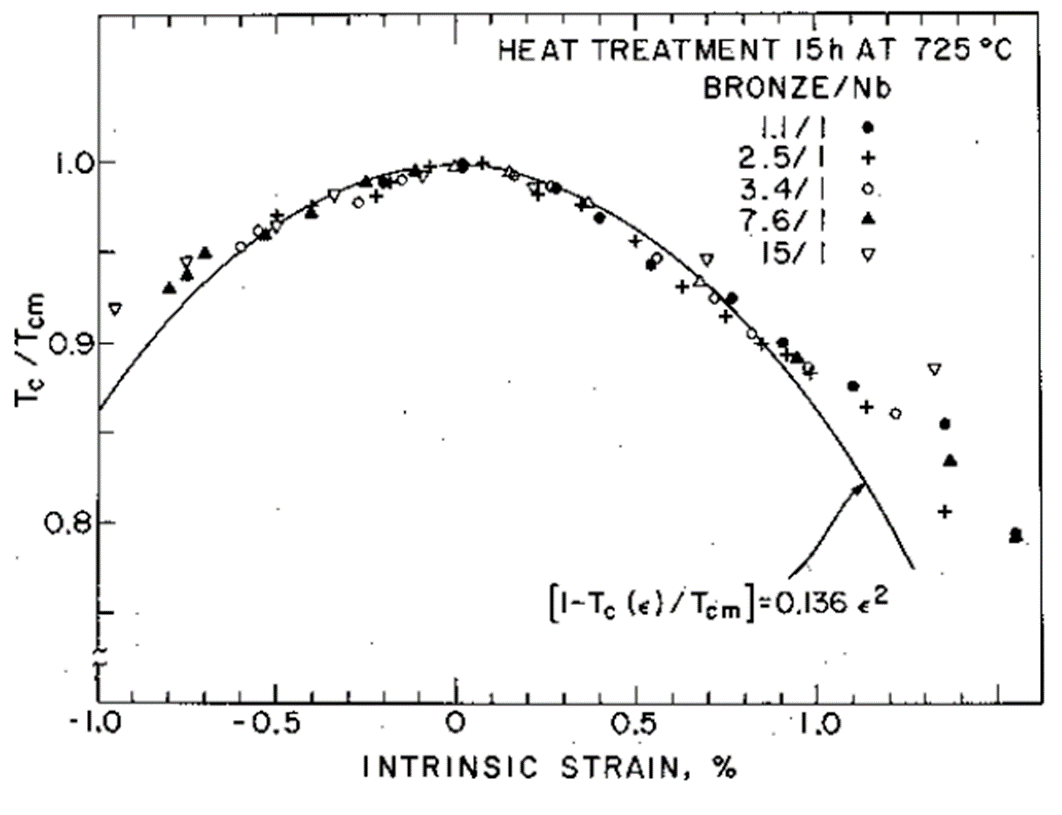
\includegraphics[width=.6\textwidth]{images/intro/Nb3SnProperties/TcvsStrain.png}
        \caption{Nb$_3$Sn's strain-dependent critical temperature for bronze processed Nb$_3$Sn wires under tension and compression~\cite{ekinStrainScalingLaw1980}.}
        \label{fig:TcvsStrain}
    \end{figure}

     \begin{figure}[htb]       
        \centering
        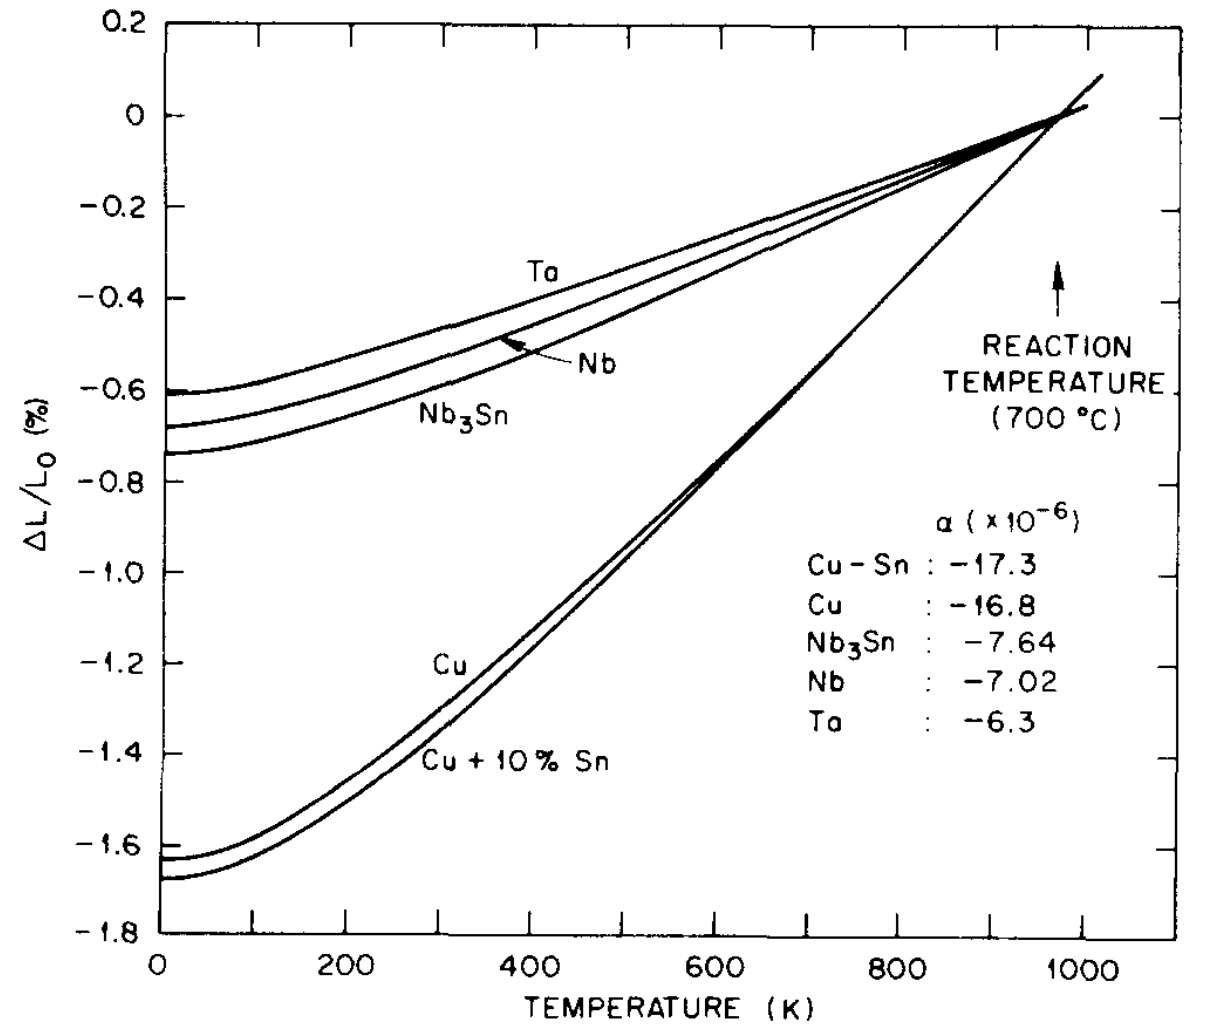
\includegraphics[width=.6\textwidth]{images/intro/Nb3SnProperties/CTECuNbNb3Sn.png}
        \caption{Coefficient of Thermal Expansion (CTE) or Cu, Nb, and Nb$_3$Sn starting with zero strain at 700~$^\circ$C~\cite{eastonPredictionStressState1980}.}
        \label{fig:CTECuNbNb3Sn}
    \end{figure}
    \FloatBarrier

\section{Microstructure}

    \subsection{Common Features of the \texorpdfstring{Nb$_3$Sn}{Nb3Sn} Microstructure}

    Nb$_3$Sn forms through solid-state grain bo undary diffusion. The resulting microstructure has been studied comprehensively in the magnet community. Example wire cross-section and microstructure are shown in (a) and (c) of~Fig.\ref{fig:Nb3SnMicrostructure}. The Nb$_3$Sn near the Sn source forms as small equiaxed grains that are high in Sn content. Nb$_3$Sn, further from the Sn source, forms as long columnar grains because the Sn is supplied at a lower rate, having to go through all the grains from the Sn source to the last Nb$_3$Sn layer. Example microstructure from a  Nb$_3$Sn thin film using the Sn vapor route can be seen in (b) of Fig.~\ref{fig:Nb3SnMicrostructure}.
    

     \begin{figure}[tbh]      
        \centering
        
\includegraphics[width=.9\textwidth]{images/Nb3Sn/Nb3SnMicrostructure.png}
        \caption[(a) Wire cross section with Nb$_3$Sn filaments~\cite{jewellInfluenceNb3SnStrand2003}, and (c) closer look at microstructure with small grains near the Sn source and large columnar grains farther from the Sn source~\cite{leeMicrostructuralFactorsImportant2008} commonly found in Nb$_3$Sn wires.]{(a) Wire cross section with Nb$_3$Sn filaments~\cite{jewellInfluenceNb3SnStrand2003}, and (c) closer look at microstructure with small grains near the Sn source and large columnar grains farther from the Sn source~\cite{leeMicrostructuralFactorsImportant2008} commonly found in Nb$_3$Sn wires. (b) Cross-section microscopy showing thin film Nb$_3$Sn grains made with the Sn vapor route~\cite{leeGrainboundaryStructureSegregation2020}. }
        \label{fig:Nb3SnMicrostructure}
    \end{figure}
    \FloatBarrier


    \subsection{Grain Boundaries}

    Grain boundaries affect Nb$_3$Sn performance differently depending on the application. In magnets, grain boundaries provide beneficial flux pinning at high fields. In RF cavities operating near zero field, grain boundaries contribute to residual surface resistance. Because grain boundaries are narrow ($\sim$5~nm), transmission electron microscopy (TEM) is required to resolve their composition. Figure~\ref{fig:TEMHotBronze} shows a hot-bronze film on a bronze substrate with Cu impurities segregated at the grain boundaries.

    \begin{figure}[tb]
        \centering
        
\includegraphics[width=\textwidth]{images/Bronze/TEMHotBronze.png}
        \caption{TEM image from a hot-bronze film on a bronze substrate, where Cu was found at the edge of some of the grain boundaries.}
        \label{fig:TEMHotBronze}
    \end{figure}

    \subsubsection{Accelerator Applications: Minimizing Grain Boundary Losses}
    
    Solid-state diffusion routes can trap impurities such as Cu and excess Sn in Nb$_3$Sn grain boundaries. When the grain boundary width approaches the coherence length ($\sim$3~nm), these impurities significantly obstruct supercurrent flow. In RF cavities, this increases the residual resistance $R_0$. \citeauthor{leeGrainboundaryStructureSegregation2020}~\cite{leeGrainboundaryStructureSegregation2020} showed that annealing at 1100~°C for 3~hours drives Sn out of grain boundaries, increasing the quality factor from $2\times10^{10}$ to $3\times10^{10}$ without degrading other properties (Fig.~\ref{fig:QfactorSngrain}). Ab initio calculations have confirmed that grain boundary impurities degrade superconducting properties in the Cu-Nb-Sn system~\cite{kelleyInitioTheoryImpact2020}.
    
    \begin{figure}[tb]
    \centering
        \includegraphics[width=\textwidth]{images/intro/Nb3SnProperties/QfactorSngrain.png}
        \caption{Q factor measurements showing improved performance in samples with Sn removed from grain boundaries via high-temperature annealing~\cite{leeGrainboundaryStructureSegregation2020}.}
        \label{fig:QfactorSngrain}
    \end{figure}

    
    \subsubsection{High-Field Applications: Enhancing Flux Pinning}

    For high-field applications, grain boundaries serve as beneficial flux pinning centers. Pinning force scales inversely with grain size ($F_p \propto 1/d$)~\cite{scanlanFluxPinningCenters1975}, so higher grain boundary density reduces Campbell resistance $R_C$ in applied fields. The pinning mechanism arises because grain boundaries locally suppress the superconducting order parameter, creating sites that interact strongly with vortex cores~\cite{gurevichNonlocalJosephsonElectrodynamics1992, gurevichTimeScalesFlux1993, gurevichAnisotropicFluxPinning1994}. These models predict that vortices depin at currents less than 10\% of the current circulating within vortex cores, so the current-blocking effect of grain boundaries discussed in the previous section is negligible for pinning applications. The trade-off is that increased grain boundary density may raise the residual resistance $R_0$ at zero field.
    
    %The Nb$_3$Sn magnet community exploits this effect, attributing high critical current density $J_c$ to increased grain boundary density through grain refinement~\cite{cooleyShiftFluxpinningForce2001}. Strategies include doping and low-temperature heat treatments to suppress grain growth. Early work in the 1980s--1990s investigated oxidation effects on pinning~\cite{braginskiFormationA15Phase1986, rumanerRoleOxygenZirconium1994}, with recent studies using internal oxidation via Sn-oxide powder to enhance pinning through controlled oxygen incorporation at grain boundaries~\cite{Sun:2023nwg, Xu:2023wai}. This remains an active research area, as CERN's High-Luminosity LHC upgrade requires higher $J_c$ performance at elevated operating temperatures (from 2 to 4~K).
    
    \subsubsection{Implications for Axion Detection}
    
    For axion detector cavities operating in 9~T fields, grain boundaries present a trade-off: they provide beneficial flux pinning (reducing $R_C$) but may increase residual resistance ($R_0$). The optimal microstructure depends on which loss mechanism dominates at the operating frequency, temperature, and field. Key open questions include whether films with smaller grains improve high-field performance through enhanced pinning, and whether Cu impurities in grain boundaries degrade performance in applied fields as they do at zero field.
    
    %Other groups that grow Nb$_3$Sn on copper that don’t use the Cu-Sn-Nb ternary reaction have problems with homogeneity and low Sn concentration~\cite{Ilyina-Brunner:2019iay, Tan:2020hmh, xiaoAnnealingStudyProperties2021}. 

 
    
    
    %However, some new recipes show some promise~\cite{Ilyina-Brunner:2019iay} (\cite{piraProgressEuropeanThin2023}). 


    %I have analyzed the material's microstructure using a scanning electron microscope (SEM) with a resolution of 50nm. I use the focused ion beam (FIB) to cut into my material and examine the cross-section with SEM. I can also cut out a thin lamella $50 \si{nm}$ and mount it to a transmission electron microscope (TEM) for later sub-angstrom analysis. This higher-resolution microscope helps identify crystal structures, nanoprecipitates, impurities at grain boundaries, and much more. Energy-enable us to visually analyze the material's microstructur dispersive spectroscopy (EDS) can be used with the SEM or TEM to analyze the elemental concentrations in the material. These microscopes help us visually analyze the microstructure of the material.

   %X-ray diffraction is a valuable tool for determining the crystal structure of your material and measuring lattice spacing, which is a measure of strain. 

    %Superconducting measurements can be made on samples to determine the material's critical temperature. This is a direct measurement of multiple properties in one, such as strain and the percentage of Sn in Nb$_3$Sn. 
    
    %\section{Challenges}

    
\section{Fabrication Methods for Films and Coatings}\label{sec:coatings}
    
    Due to the low toughness and thermal conductivity of Nb$_3$Sn, it is neither practical nor favorable to make a cavity from bulk Nb$_3$Sn. Nb$_3$Sn, therefore, must be fabricated as a thin film, and ideally on a thick, high thermal conductivity metal. There are many different techniques to deposit Nb$_3$Sn as a thin film. The industry-standard accelerator method, the Sn vapor method~\cite{peinigerNb3SnSUPERCONDUCTINGACCELERATORS1989,posenMeasurementHighQuality2022}, is the most developed Nb$_3$Sn thin film process, but is limited to Nb substrates. Other methods, such as the ternary route explored in this work, enable thin film fabrication on Cu substrates, which also present challenges.

    For Nb$_3$Sn fabrication to be compatible with Cu substrates, the reaction temperature must be well below the melting temperature (1084 $^\circ$C) of Cu. High-temperature processes promote annealing and recrystallization, which cause the substrate to lose strength~\cite{okudaFabricationTestingLband1991}. This temperature constraint divides Nb$_3$Sn axion detector cavity fabrication methods into two categories: high-temperature routes limited to Nb substrates ($>950~^\circ$C), and low-temperature routes compatible with Cu substrates ($<750~^\circ$C). 

    \subsection{Substrate Requirements}

    Cu is an ideal substrate for maintaining an isothermal cavity environment due to its high thermal conductivity, which prevents thermal gradients during operation. However, fabricating Nb$_3$Sn on Cu presents a critical challenge: the Cu substrate acts as a Sn sink, depleting Sn from the Cu-Sn/Nb$_3$Sn reaction zone. Since $T_c$ depends strongly on Sn content (Fig.~\ref{fig:TcvsSnMoore}), this depletion degrades superconducting performance. A diffusion barrier of refractory metals (Ta, Mo, Nb, W) between the Cu substrate and the Cu-Sn source layer can block Sn migration while maintaining thermal contact.
    
    Substrate surface roughness and cleanliness critically affect thin film quality, since deposited films replicate the underlying surface morphology. The challenge intensifies when underlying layers undergo structural changes during heat treatment, including recrystallization and grain growth. For example, if a Cu-Sn source layer sits between the Cu substrate and the Nb$_3$Sn film, the Cu-Sn layer will undergo phase transformations and volume changes during the reaction (Sec.~\ref{sec:NbCuSn}). These structural rearrangements can induce strain, surface roughness, or, in severe cases, cracking and delamination of the overlying Nb$_3$Sn film. The choice of substrate and its effect on the thin film must be carefully considered when selecting a method and recipe for thin film fabrication.
    
    \subsection{High-Temperature Routes (Nb Substrates Only)}
    
    \subsubsection{Sn Vapor Method} \label{sec:Snvapordetail}

    The Sn vapor method is the most mature route for Nb$_3$Sn thin film fabrication~\cite{peinigerNb3SnSUPERCONDUCTINGACCELERATORS1989,posenMeasurementHighQuality2022}. Bulk Nb cavities are exposed to Sn vapor at elevated temperatures, forming Nb$_3$Sn through solid-state diffusion. Thermodynamically, the binary Nb-Sn reaction requires temperatures above 950~$^\circ$C to destabilize competing phases (Nb$_6$Sn$_5$ and NbSn$_2$) and stabilize stoichiometric Nb$_3$Sn~\cite{xuxingchenReviewProspectsNb3Sn2017}. However, kinetic limitations necessitate a reaction temperature near 1100~$^\circ$C to drive the reaction to completion. This method has achieved the highest quality factors ($Q_0 \sim 10^{11}$) at zero field among Nb$_3$Sn fabrication techniques for accelerator applications~\cite{Posen:2018zjb}.

    The Sn Vapor method has good surface coverage, compared to line-of-sight deposition methods. This enables a relatively uniform coating on the inside of complex geometries. However, since the wettability of Sn on Nb is poor~\cite{heinSuperconductingIntermetallicCompounds1973}, tin chloride (SnCl$_2$) gas is used to improve wetting and help seed Nb with Sn atoms. This initiates the nucleation of initial Nb$_3$Sn growth, which is further driven by a post-reaction at 1100 $^\circ$C. The resulting Nb$_3$Sn has sharp superconducting transitions ($\Delta T_c < 1$~K) with critical temperatures near the optimal value of $T_c\approx18$~K~\cite{Posen:2018zjb}.
    
    The Sn vapor method is continuing to improve, advancing toward higher accelerating gradients~\cite{posenNb3SnSuperconductingRadiofrequency2022, Posen:2018zjb, Posen:2020kei}. Recent work by Viklund et al. demonstrated that cavities can be mechanically polished to remove defective Nb$_3$Sn layers and recoated to achieve performance equal to or exceeding the original coating~\cite{Viklund:2023uxj, Viklund:2023nlq, Viklund:2024lew}. Still, this process has shortcomings, including poor uniformity and the presence of Sn domains near the center of the Sn seed~\cite{Viklund:2023uxj}.

    Jefferson Lab and Fermilab have developed hybrid approaches that retain the good superconducting properties of the Sn vapor method while incorporating Cu for thermal management. They use Cu cooling clamps, and electroform Cu in a shell around the completed Nb$_3$Sn/Nb cavity. These modifications sufficiently improve thermal conductivity to enable cryocooler operation (rather than liquid helium), thereby reducing operating costs. However, thermal performance remains limited due to the significant distance (mm-scale) between the Nb$_3$Sn film and the outer Cu shell~\cite{ciovatiDesignCwLowenergy2018, posenNb3SnSuperconductingRadiofrequency2022}. The Cu clamping approach may be a feasible way to increase thermal conductivity for axion detector cavities. However, the room is very limited in the bore of a magnet, and the Cu clamp occupies valuable bore space that could be better used to increase the axion-photon cross section (more cavity volume) than to increase thermal conductivity.
        
    \subsubsection{Nb-Sn Multilayer Sputtering}
    
    In another high-temperature method, Nb and Sn are separately deposited in alternating layers using sputtering and a Nb substrate, followed by a reaction~\cite{vandenbergNewPhaseFormation1985}. The short diffusion distances between the Nb and Sn layers allow a slightly lower reaction temperature of 950 $^\circ$C, rather than the 1100~$^\circ$C required by the Sn vapor method. A full 2.6 GHz accelerator cavity has been coated with a cylindrical magnetron sputtering system~\cite{Shakel:2023cdz}, and reached $Q = 1.1 \times10^9$. This method has not achieved the performance levels of the Sn vapor method.

    \subsection{Low-Temperature Routes (Cu Substrate Compatible)}

    
    \subsubsection{Cu Compatible Nb-Sn Routes}\label{sec:StoichiometricDetail}
    
    The diffusion path between Nb and Sn can be reduced even further using a stoichiometric Nb$_3$Sn target or co-sputtering Nb and Sn simultaneously. This allows for Nb$_3$Sn fabrication on Cu substrates with a binary Nb-Sn route at temperatures around $700$~°C. Co-sputtering methods suffer from non-uniformity, off-stoichiometry, and Sn islands on the film's surface~\cite{Tan:2020hmh}. Additionally, films on Cu substrates cannot be post-reacted at the high temperatures ($>950$°C) typically used to optimize Nb$_3$Sn stoichiometry and microstructure after deposition. The as-deposited film is essentially final, requiring precise control of deposition parameters since deficiencies cannot be corrected through subsequent heat treatment.
    
    \citeauthor{Ilyina-Brunner:2019iay} at CERN uses Nb$_3$Sn stoichiometric targets to deposit on Cu, and they found large Cu inclusions on the surface of the Nb$_3$Sn~\cite{Ilyina-Brunner:2019iay}. These Cu inclusions are detrimental to RF properties, so subsequent experiments used a thick diffusion barrier between the Cu substrate and Nb$_3$Sn film to prevent Cu diffusion to the surface.
    
    %\begin{figure}        
     %   \centering
     %   
\includegraphics[width=.5\textwidth]{images/Metallurgy/Cu inclusions.png}
     %   \caption[EDS map of Cu inclusions on surface]{EDS mapping of a Cu inclusion on the surface of a Nb$_3$Sn film. Scale bars represent 1 \si{\um}~\cite{Ilyina-Brunner:2019iay}.}
    %    \label{fig:Cu inclusions}
    %\end{figure}
    
    Recent progress~\cite{fonnesuRecipeOptimizationSRF2025, piraProgressEuropeanThin2023} using optimized recipes with a stoichiometric target has shown a world record low surface resistance $R_s\approx 7$~\unit{n\ohm} using a Nb substrate quadrupole resonator (QPR) sample. \citeauthor{Ilyina-Brunner:2019iay} have near-term plans of coating a full cavity with their recipe, and have results showing that their process has higher pinning properties than those of the Sn vapor route~\cite{fonnesuRecipeOptimizationSRF2025}. This is the first result showing that Nb$_3$Sn can be fabricated with a non-Sn vapor method and display competitive properties in specific applications.
 
    Reza et al. at Daresbury noted~\cite{valizadehSynthesisNbAlternative2022, turnerFacilityCharacterisationPlanar2022, turnerInvestigationMagneticField2026} that the divergence of the sputtered plume of material from a planar magnetron was sufficient to coat the walls of a cavity resonator by simply moving the magnetron along the cavity axis, where the sputter target plane is perpendicular to the axis. This avoids complications of cylindrical magnetrons that sputter radially. An advantage of the planar magnetron is more efficient cooling, which allowed the Daresbury team to heat the cavity wall without overheating the sputter source. They have been able to make good-quality films with this process and aim to test full cavities soon. With these low-temperature binary Nb-Sn reactions, the energy and rate of the deposition are crucial for achieving optimal stoichiometry.
    
    \subsubsection{Cu-Nb-Sn Route: Electrochemical Cu-Sn Process}
    
    The ternary route leverages technology developed for Nb$_3$Sn high-field magnets. Using a pseudo-binary reaction between a Cu-Sn compound and Nb avoids the unfavorable superconducting compounds and lowers the practical Nb$_3$Sn reaction temperature. This is often termed the bronze route~\cite{suenagaChemicalCompositionsGrain1983, tachikawaHighFieldNb3SnSuperconductors1997} in reference to the alpha Cu-Sn phase called bronze.

    The bronze route has been successfully applied to Nb cavities by \citeauthor{luDevelopmentPerformanceFirst2022} in China~\cite{luDevelopmentPerformanceFirst2022}. A bronze layer was electroplated onto the inner surface of a Nb cavity and subsequently reacted, achieving a quality factor of $1.2 \times 10^9$. This Chinese group also coated Cu substrate samples using the same electrochemical process, in which they first sputtered a thick 5~$\mu$m Nb layer onto the Cu substrate, electroplated Cu-Sn, heat-treated in vacuum at 700~$^\circ$C, and then removed the Cu-Sn layer by electropolishing~\cite{Lu:2023wyr}. The group hopes to extend the process to a full-sized Cu cavity. The bronze route can also be used to fabricate multiple electroplated layers of alternating Cu and Sn~\cite{franzSYNTHESISNbSnCOATINGS2017}. The resulting films using this method have characteristics similar to those of the above electroplated Cu-Sn films.

    The advantage of the electrochemical processing method is that it can uniformly coat complex geometries. However, one potential pitfall of this method is the large impurity concentration created when using aqueous electrochemical solutions, which introduce oxygen and organic contaminants into the Cu-Sn fil, resulting in broader superconducting transitions ($\Delta T_c = 1.5-4$~K)~\cite{luDevelopmentPerformanceFirst2022, luElectrochemicalThermalSynthesis2021, luImpactCuSn2025}.
    
    \subsubsection{Cu-Nb-Sn: Thermal Evaporation Cu-Sn Process (This Work)}\label{sec:ourworkdescribe}
    
    This dissertation explored the deposition of Cu-Sn layers by thermal evaporation. This work adds to studies conducted at the Applied Superconductivity Center (ASC) in the early 2000s~\cite{cooleyShiftFluxpinningForce2001}, in which Nb was deposited on bronze samples. The pinning force was analyzed and found to be higher in films with $20-50$~nm grains (hot-bronze films) than in films with $50-250$~nm grains (post-reacted films).

    The pseudo-binary reaction path is very similar to the electrochemical process described above, except that thermal evaporation is used to deposit the Cu-Sn. Evaporation allows control of the Sn concentration in the range $10-40$~at.\% Sn, and since it takes place in a high-vacuum environment, impurities from aqueous solutions are avoided. Narrow superconducting transitions ($\Delta T_c \sim 1 $~K) have been obtained. Obtaining good Nb$_3$Sn films critically depends on the cleanliness of the environment during deposition and reaction~\cite{withanageRapidNbSn2021}. The sputter chamber for Nb deposition and the thermal evaporator for Cu-Sn deposition both use vacuum systems designed to limit oxygen and carbon from entering the film. This work employed two line-of-sight physical vapor deposition techniques: thermal evaporation and magnetron sputtering.

    %impurity concentration in the Cu-Sn film, which results in sharper superconducting transitions ($\Delta T_c \sim 1$~K) compared to electrochemical routes ($\Delta T_c = 1.5-4$~K). 

    Two variants using this thermal evaporation approach were developed. The first is a post-reaction solid-state diffusion technique. This method requires a Cu-Sn film in contact with a Nb layer, where Sn diffuses out of the Cu-Sn film into the Nb, forming Nb$_3$Sn at the Cu-Sn/Nb interface. The speed of this reaction is limited by the grain boundary diffusion rate of Sn through the Nb$_3$Sn grains. The second variant is a vapor reaction method termed the hot-bronze technique. A Cu-Sn film is heated, and Nb atoms arrive and immediately react with a high concentration of Sn vapor right above the Cu-Sn film~\cite{withanageRapidNbSn2021}. During Cu-Sn heating, the bronze target surface turns silver, confirming its Sn-rich composition. Hot-bronze films can be further improved with an additional post-reaction heat treatment. The Sn in the remaining Cu-Sn layer continues to feed the Nb$_3$Sn during this anneal, further saturating the Nb$_3$Sn grains and increasing $T_c$. The resulting film microstructure is fundamentally different between the two variants: the hot-bronze variant shows large columnar grains spanning the film thickness, whereas the post-reaction method shows standard equiaxed grains near the Sn source and columnar grains farther from the Sn source.

    
    \subsection{Summary of Fabrication Techniques}
    
    All the fabrication methods are listed in Table~\ref{fig:Nb3SnFabrication2}. 
    
    %The Sn vapor method achieves the highest quality factors for accelerator applications ($Q \sim 10^{11}$) but limited to Nb substrates. The stoichiometric target method demonstrates excellent surface resistance on Cu substrates and has shown superior pinning for high-field applications. However, they face challenges with this method's inability to effectively post-react the samples to enhance superconducting properties further. However, they have shown promising results with careful optimizations of the ad-atom rate and energy. The stoichiometric method's results represent a significant milestone for Cu-compatible Nb$_3$Sn fabrication.
    
    %Electrochemical bronze routes have successfully demonstrated full-cavity coating capability and excellent coverage on complex geometries. However, aqueous processing introduces oxygen and organic impurities, resulting in broad $T_c$ transitions ($\Delta T_c \sim 1.5-4$ K), indicating compositional inhomogeneities throughout the film thickness. Our thermal evaporation Cu-Sn route allows post-reaction at a lower temperature, enabling film optimization after deposition while remaining Cu-compatible. Our route also allows the fabrication of films with low impurity content, thereby yielding sharp superconducting transitions. A new microstructure with small grains is also accessible via the hot-bronze route, which may help optimize pinning forces in future high-field studies. 
    
    \begin{table}[ht]      
    \centering
        \caption{Comparison of Nb$_3$Sn fabrication methods showing reaction temperature, equipment requirements, substrate compatibility, and key performance characteristics~\cite{posenNb3SnSuperconductingRadiofrequency2017,luElectrochemicalThermalSynthesis2021, sayeedFabricationSuperconductingNb3Sn2023, schaferKineticallyInducedLowtemperature2020, Ilyina-Brunner:2019iay, withanageRapidNbSn2021}.}
    
\includegraphics[width=.9\textwidth]{images/Nb3Sn/Nb3SnFabrication2.png}
    \label{fig:Nb3SnFabrication2}
    \end{table}
    \FloatBarrier

    \subsection{Future Directions}

    The Nb$_3$Sn thin-film cavity community has adopted many different approaches that trade off benefits and constraints. Future work might consider combining the strengths of various approaches to overcome weaknesses. For instance, the fabrication process could start with an electrochemical Cu-Sn seed layer to achieve uniform coverage and increased Sn wettability, and then deposit a higher-Sn, impurity-free Cu-Sn film via thermal evaporation. Collaborative development may help accelerate Nb$_3$Sn fabrication towards a reproducible high-$Q$, high-field superconducting RF resonator. 